\section{Analysis of Inclusive Cross Section}

The structure function ratios $A_{UU}^{\cos\phi}$ and $A_{UU}^{\cos(2\phi)}$ were previously measured by hall-B and analyzed by Nathan Harrison.  In this dissertation we extend this previous work by calculating, validating, and applying the integrated luminosity factor necessary to transform this previous measurement into an absolute cross section.  In order to validate the integrated luminosity calculation, we have measured the cross section for inclusive electron scattering ($ep \rightarrow e'X$).  This work entailed calculating the integrated luminosity \cite{fcup-note}, measuring the electron yield in bins of $W$ and $Q^2$, and corrected these yields for acceptance effects as well as radiative effects.  The cross section is experimentally measured by combining the following factors. 

\begin{equation}
  \frac{d\sigma_i}{dW dQ^2} = \frac{1}{\Delta W_i \Delta Q^2_i} \frac{N_{obs} - N_{BG}}{\mathcal{L}} \frac{1}{A_i R_i}
\end{equation}

Here $W$ is the invariant mass of the virtual photon and target system ($\gamma^* + p$), calculated as $W = \sqrt{M_{p}^{2} - Q^2 + 2{p^\mu} q_{\mu}}$.  In the equation above, $A_i$, and $R_i$ refer to the acceptance and radiative correction in the i-th bin.  This cross section is experimentally well studied, and our comparison with existing models shows that our measurement is consistent.  This gives us a trust in our electron identification, as well as our luminosity (used later to scale the SIDIS data).  The inclusive scattering measurement will be described below.

\subsection{Calculation of Integrated Luminosity}
During running of experimental data taking beam charge accumulates on the Faraday Cup.  The accumulated charge is written out into the data files for later processing.  By summing the charge on the Faraday cup over the entire set of files used in the analysis, the total accumulated charge $\Delta Q$ can be calculated.  The incoming number of electrons is then $N_e = \Delta Q/e $.  The integrated luminosity is then; 

\begin{equation}
  \mathcal{L} = \frac{\Delta Q l_t \rho}{e}
\end{equation}

Care is taken when calculating the integrated luminosity.  In the case that there is a time period where charge is accumulating and events are not, this section is skimmed out of the datafile, and the charge is not added.  In the case that there is no charge accumulating but events are occuring, these events are discarded.  Plots for every run used can be found at \cite{fcup-website}.

\easyFigure{image/charge_37844.png}{The charge accumulated per scalar entry for run 37844.}

\subsection{Acceptance Corrections}
A fraction of the events which occur are not captured by the detector due to two main reason: 

\begin{enumerate}
  \item The detector components do not have 100\% efficiency.
  \item The detector has geometric holes and obstructions, through which particles can/can not pass.
\end{enumerate}

Some of these effects (holes/obstructions) can be taken into consideration using fiducial cuts during the particle identification stage.  Other effects  have to be taken into account by correcting for the detectors not perfect acceptance.  This is done by creating a computer model of the detector, as realistically as possible.  Inclusive events (with radiative effects) are then simulated leaving the target and propagating through the magnetic field, hitting the detectors of CLAS.  These results can then be used to form the correction factor $A = N_{rec}/N_{gen}$ in every bin.  

\subsection{Radiative Corrections}
It is not uncommon for electrons to emit a real photon in the initial or final state of the interaction.  These radiations alter the event kinematics and must be removed in order to present Born cross sections (nature provides us with the radiated cross section).  This is done by modeling the inclusive reaction with and without radiative effects and comparing the results.  The correction factor $R = N_{rad}/N_{no rad}$ can be constructed from a sufficient event generator(in this analysis we use \texttt{keppel\_rad} and \texttt{keppel\_norad}).  

\subsection{Comparison to Model}
Our result is compared to a parametrization of the resonance region between $W \in [1.1, 2.0]$ \cite{theses-keppel:1994}.  This parametrization was originally developed at SLAC by Cynthia Keppel and has been improved using data from Hall-C over time.  Over the majority of the kinematics the result is within 5\% of the model value.  This contamination is in large part due to elastic events which persist in the lower and higher $W$ parts of the measurement.  Despite this, the average discrepancy over the entire phase-space of the measurement is included as a quoted uncertainty on the integrated luminosity.  

%\begin{figure}
%  \centering
%  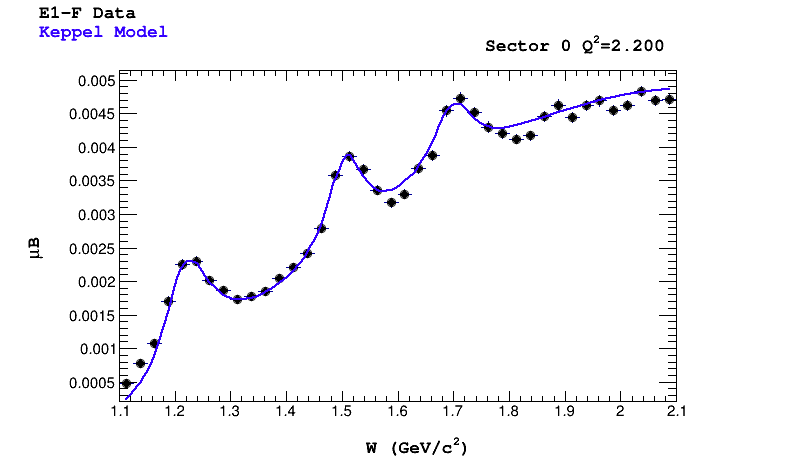
\includegraphics[width=5cm]{image/compareDataModelSector0Slice2.png}
%  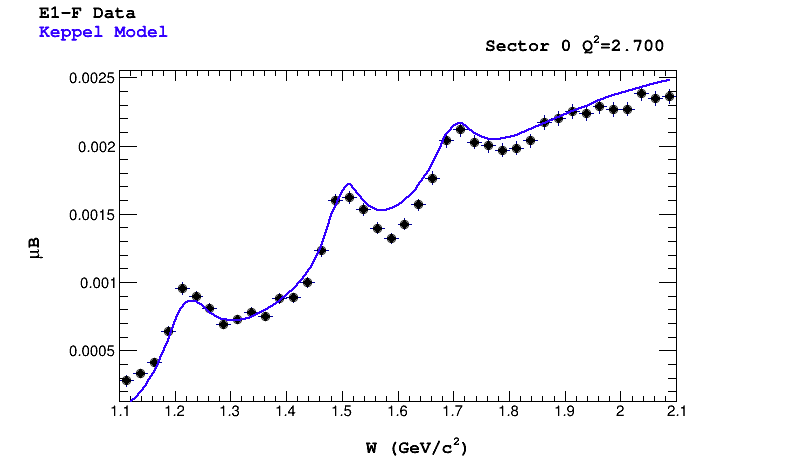
\includegraphics[width=5cm]{image/compareDataModelSector0Slice4.png}
%  \caption{Our cross section result compared with Keppel's model.}
%\end{figure}

%\begin{figure}
%  \centering
%  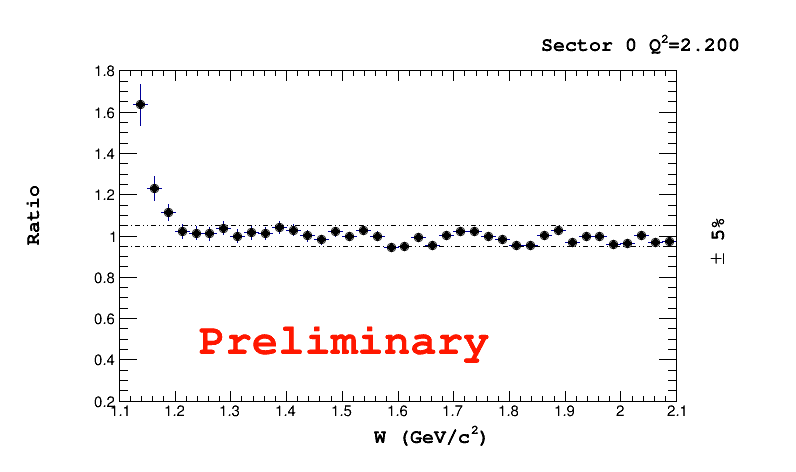
\includegraphics[width=5cm]{image/crossSectionRatioSector0Slice2.png}
%  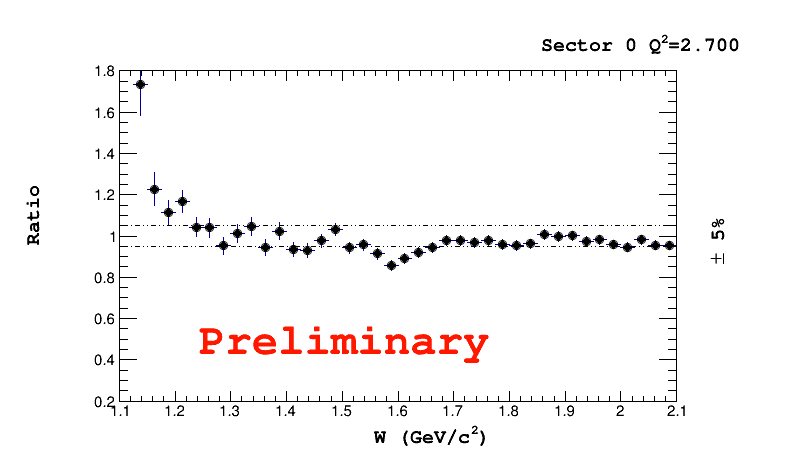
\includegraphics[width=5cm]{image/crossSectionRatioSector0Slice4.png}
%  \caption{Ratio of data to Keppel model.}
%\end{figure}

%%%%%%%%%%%%%%%%%%%%%%%%%%%%%%%%%%%%%%%%%%%%%%%%%%%%%%
%
%     Too many figures for this short document.
%
%%%%%%%%%%%%%%%%%%%%%%%%%%%%%%%%%%%%%%%%%%%%%%%%%%%%%%
\easyFigure{image/compareDataModelSector0Slice2.png}{Our cross section result compared with Keppel's model.}
%\easyFigure{image/crossSectionRatioSector0Slice2.png}{Our cross section result compared with Keppel's model.}

